\documentclass[12pt,a4paper]{article}
\usepackage[utf8]{inputenc}
\usepackage[english]{babel}
\usepackage{amsmath}
\usepackage{amsfonts}
\usepackage{amssymb}
\usepackage{graphicx}
\usepackage{hyperref}

\usepackage{dsfont}

\author{José Antonio García Hernández}
\title{2-dimensional lattice SU(2) gauge field theory}
\begin{document}
\maketitle
\section{Introduction}
$U \in \text{SU}(2)$.

\begin{equation}
	\label{eq:SU2_element}
	U = \begin{pmatrix}
		a & b \\
		-b^* & a^*
	\end{pmatrix}
\end{equation}
where $a, \ b \in \mathbb{C}$ and $|a|^2 + |b|^2 = 1$.


Continuum action
\begin{equation}
	\label{eq:continuum_action}
	S[A] = \frac{1}{2g^2} \int d^4x \, \text{Tr} \left[ F_{\mu\nu}(x)F_{\mu\nu}(x)\right].
\end{equation} 

Plaquette variable
\begin{equation}
	\label{eq:plaquette}
	U_{\mu\nu}(x) = U_{\mu}(x)U_{\nu}(x+\hat{\mu})U_{\mu}^{\dagger}(x+\hat{\nu})U_{\nu}^{\dagger}(x) 
\end{equation}


Lattice action
\begin{equation}
	\label{eq:wilson_action}
	S[U] = \frac{\beta}{N}\sum_x \sum_{\mu < \nu} \text{Re}\ \text{Tr} \left[\mathds{1} - U_{\mu\nu}(x) \right],
\end{equation}
where $\beta = \frac{2N}{g^2}$.

Sum of plaquette variables
\begin{equation}
	\label{eq:Sp}
	S_{\text{P}} = \frac{1}{N} \sum_x\sum_{\mu < \nu} \text{Re}\ \text{Tr} [U_{\mu\nu}(x)]
\end{equation}
we define
\begin{equation}
	\label{eq:Ep}
	E_{\text{P}} =\frac{ \langle S_{\text{P}} \rangle}{D V}
\end{equation}
where $V=L^d$ is the volume of the lattice and $D = \frac{d(d-1)}{2}$ is the number of planes of rotation.

Staples
\begin{equation}
	\label{eq:staples}
	\Sigma_{\mu}(x) = \sum_{\nu \neq \mu} \left[ U_{\nu}(x)U_{\mu}(x+\hat{\nu})U_{\nu}^{\dagger}(x+\hat{\mu}) + U_{\nu}^{\dagger}(x-\hat{\nu})U_{\mu}(x-\hat{\nu})U_{\nu}(x+\hat{\mu}-\hat{\nu})\right]
\end{equation}


The change in the action  by a local update when changing $U_{\mu}(x) \to U'_{\mu}(x)$ is
\begin{equation}
	\label{eq:DS}
	\Delta S = -\frac{\beta}{N} \text{Re } \text{Tr} \left[ \left( U'_{\mu}(x) - U_{\mu}(x) \right)\Sigma_{\mu}^{\dagger}\right]
\end{equation}

\section{Algorithms}

We implemente three local update algorithms, namely, Metropolis, Glauber and Heathbath.

\subsection{Metropolis}
\begin{enumerate}
	\item Given some gauge field configuration, we go through all the lattice points in a lexicographic way. At each point $x$ in the $\mu$ direction we generate a random SU(2) matrix $U'_{\mu}(x)$.
	
	\item We compute the sum of the staples and compute the change of the action according to eq.\ \eqref{eq:DS}. We generate a uniform random number $r\in [0,1)$ and accept the change if $r \leq p$, where $p$ is
	\begin{equation}
		p = \min (1, \exp(-\Delta S)).
\end{equation}	 
\end{enumerate}

\subsection{Glauber}
\begin{enumerate}
	\item Given some gauge field configuration, we go through all the lattice points in a lexicographic way. At each point $x$ in the $\mu$ direction we generate a random SU(2) matrix $U'_{\mu}(x)$.
	
	\item We compute the sum of the staples and compute the change of the action according to eq.\ \eqref{eq:DS}. We generate a uniform random number $r\in [0,1)$ and accept the change if $r \leq p$, where $p$ is
	\begin{equation}
		p = \frac{1}{e^{\Delta S} + 1}.
\end{equation}	 
\end{enumerate}

\subsection{Heatbath}\label{sec:heatbath}
In the heatbath algorithm we need to generate an update $X\in\text{SU}(2)$
	 \begin{equation}
	 	X = \begin{pmatrix}
	 		 x_0 + ix_1 & x_2 + ix_3 \\
	 		-x_2 + ix_3 & x_0 - ix_3
	 	\end{pmatrix}
	 \end{equation}
	 where $x_0, x_1, x_2,x_3 \in \mathbb{R}$
 following the distribution
\begin{equation}
	dP(X) = \frac{1}{2\pi^2} d\cos\theta\, d\varphi\, dx_0\, \sqrt{1-x_0^2}e^{a\beta x_0}
\end{equation}
\begin{enumerate}
\item Given some field configuration ata point $x$ and directin $\mu$, we find the sum of staples $\Sigma_{\mu}(x)$ in eq.\ \eqref{eq:staples}, we compute $a = \sqrt{\det \Sigma_{\mu}(x)}$, and set $V = \Sigma_{\mu}(x)/a$
	\item We generate $X$ as follows:
	\begin{enumerate}
	\item	We generate three random numbers $u_i$, $i = 1,\ 2,\ 3$ in the interval [0,1) uniformly distributed and take $r_i = 1 - u_i$. Then
		 \begin{equation}
		 	\lambda^2 = -\frac{1}{2a\beta}\left(\log(r_1) + \cos^2(2\pi r_2)\log(r_3)\right).
		 \end{equation}
	\item We accept the value of $\lambda$ which obey
		\begin{equation}
			s^2 \leq 1- \lambda^2,
		\end{equation}
		where $s$ is a uniformly distributed random number in the interval [0,1).
	\item Repeat the previous two steps until a value of $\lambda$ is accepted. The accepted value gives $x_0 = 1 - 2\lambda^2$
	\item We take the norm of the vector $\vec{x} = (x_1,x_2,x_3)$ as $|\vec{x}| = \sqrt{1 - x_0^2}$.
	\item We take two uniformly distributed random numbers $\varphi\in [0,2\pi)$ and $\theta \in [0,\pi)$ and take
	\begin{eqnarray}
		x_1 & = & |\vec{x}| \cos\varphi \sin\theta \\
		x_2 & = & |\vec{x}| \sin\varphi \sin\theta \\
		x_3 & = & |\vec{x}| \cos\theta	.
	\end{eqnarray}		
	  
	\end{enumerate}
	\item Once $X$ is generated, the new link variable is $U = X V$
\end{enumerate}


\section{Results}

We present simulations results at equilibrium for the 2-d SU(2) gauge field theory. We use a square lattice with lenght $L$ volume $L^2$ and periodic boundary conditions in all directions.


We begin each simulation with a \textit{hotstart} where all link variables takes on random values.
In figure \ref{fig:L=10} we show the variable $E_{\text{P}}$ as defined in eq. \eqref{eq:Ep} for several $\beta$-values at a volume where $L=10$.

\begin{figure}
	\label{fig:L=10}
	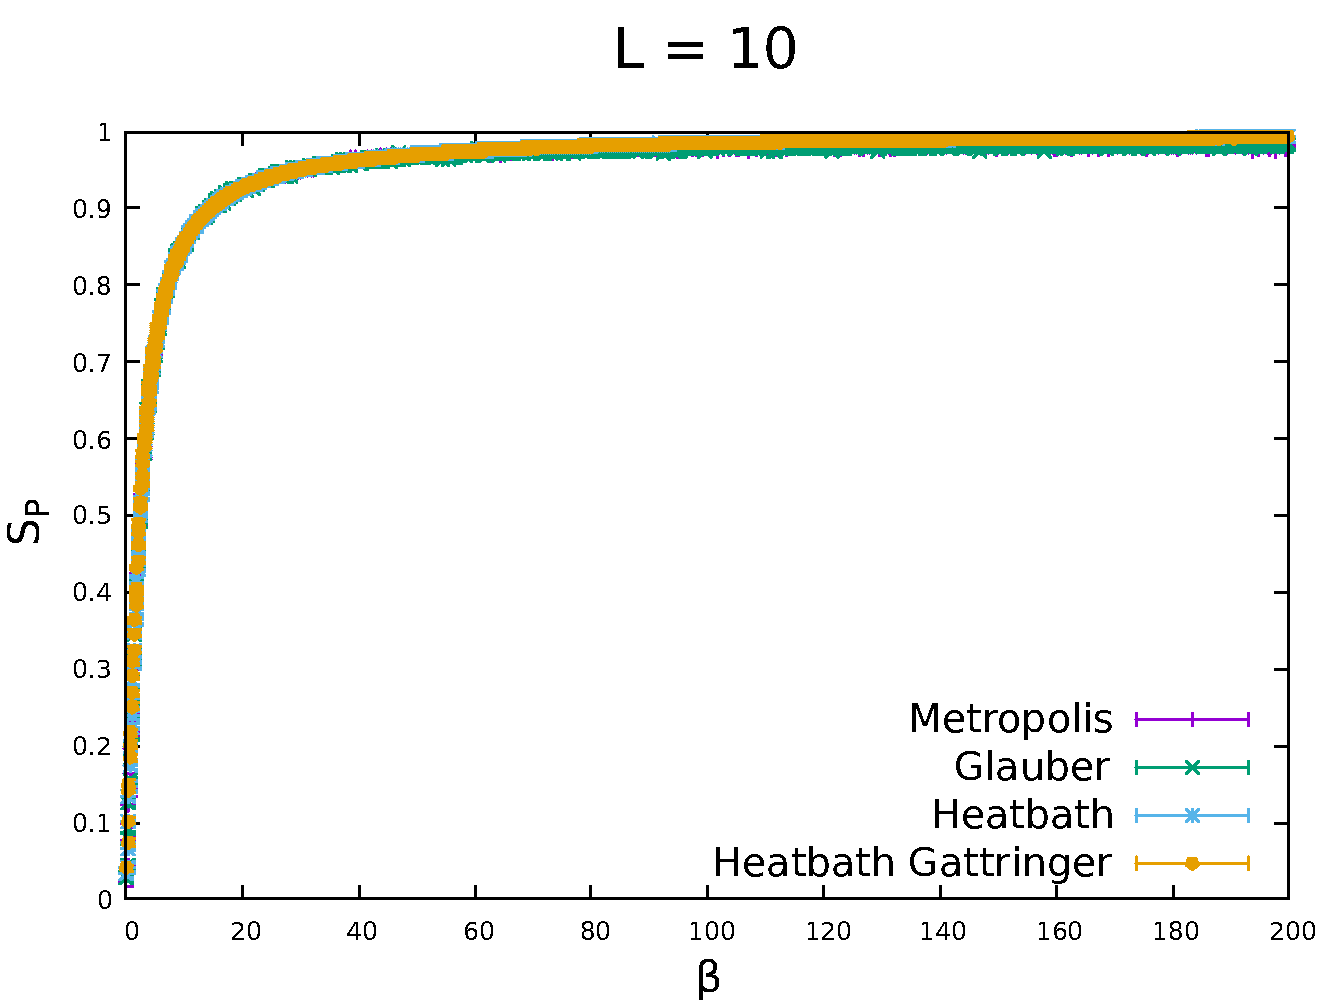
\includegraphics[scale=0.6]{../images/L=10_metropolis_glauber_heatbaths_2000points.pdf}
	\caption{Average plaquette energy density vs. $\beta = \frac{4}{g^2}$ in the two dimensional SU(2) gauge theory. According to the Mermin-Wagner theorem, continuous symmetries cannot be spontaneously broken in dimensions $d\leq 2$, therefore there is no prescence of a phase transition. We implemented three differente algorithms, Metropolis, Glauber and Heatbath. We used two equivalent implementations to generate $X$ in the heatbath algorithm, Heatbath Gattringer is the one explained in section \ref{sec:heatbath}, the other one was copied from \cite{ricker}.}
\end{figure}


\section{Acknowledgements}
The author thanks Dr.\ Wolfgang Bientholz for funding (in the form of meals) this research.

\begin{thebibliography}{99}

\bibitem{gattringer} C.\ Gattringer and C.B.\ Lang, \emph{Quantum Chromodynamics on the Lattice: An Introductory Presentation},  Lect.\ Notes Phys.\ 788 (Springer, Berlin Heidelberg 2010).

\bibitem{Gunther} F. Knechtli, M. Günther and M. Peardon, \emph{Lattice Quantum Chromodynamics Practical Essentials}, 
(Springer Briefs in Physics 2017).

\bibitem{Metropolis} N.\ Metropolis {\it et al.},
\emph{Equation of State Calculations by Fast Computing Machines},
J.\ Chem.\ Phys.\ {\bf 21} (1953) 1087.

\bibitem{Glauber} R.J.\ Glauber,
  \emph{Time-Dependent Statistics of the Ising Model},
  J.\ Math.\ Phys.\ {\bf 4} (1963) 294.
  
\bibitem{Gerber} U.\ Gerber,
  \emph{Heatbath Algorithm for the 2d U(1) Model}.
  Informal Notes. Universidad Nacional Autónoma de México, 2015.  
  
\bibitem{ricker} \url{https://github.com/alfredricker/LQCD}

\end{thebibliography}
	
\end{document}